\chapter{Vsuvka do teorie míry}
\begin{define}
	Nechť $\tau\neq\emptyset $ je libovolný systém z $ 2^\Omega$. Definujeme $\sigma (\tau)= \bigcap\limits_{\alpha}\Aa_\alpha $, kde $\Aa_\alpha$ jsou $\sigma$-algebry takové, že $\tau \subset \Aa_\alpha$. Množinu $\sigma(\tau)$ nazýváme \textbf{minimální $\sigma$-algebrou} nad systémem $\tau$.
\end{define}
\begin{define}
	Mějme $\Omega=\R^n$ a definujme $\tau:=\{\bigtimes\limits_{i=1}^n(a_i,b_i):a_i,b_i\in\R\}$. Potom $\sigma(\tau)\equal{\text{ozn}}\Bb_n$, kde $\Bb_n$ nazveme \textbf{borelovská \salg} v $\R^n$. 
Na prostoru $(\Omega,\tau)$, kde $\tau$ je topologie, pak definujeme $\sigma(\tau)=\Bb$.
\end{define}
\begin{remark}
	 $\tau$ je tedy množina všech otevřených množin v $\R^n$ a $\Bb_n$ je minimální\newline \salg~nad systémem  $\tau$. 
\end{remark}
\begin{example}
	$\Bb_n$ je bohatá a obsahuje například i
	\begin{enumerate}[a)]
		\item $\{c\}=\bigcap\limits_{n=1}^{+\infty} (c-\frac{1}{n},c+\frac{1}{n}) $
		\item $\Q, (\R\setminus\Q)$
		\item A otevřená v $\R^1$ $\Bigl(A=\bigcup\limits_{i=1}^{n,+\infty}(a_i,b_i)\Bigr)$
		\item A uzavřená v $\R^1$
	\end{enumerate}
\end{example}
\begin{define}
	Funkce $g:\Omega\to \R^n$ se nazývá \textbf{$\Aa$-měřitelná}, pokud $(\forall B \in \Bb_n)\bigl(g^{-1}(B) \in \Aa\bigr)$. Pokud $\Aa$ je borelovská \salg, potom $g$ nazýváme \textbf{borelovsky měřitelnou} funkcí.
\end{define}
\begin{define}
	Mějme funkci $\X:(\Omega,\Aa)\to (\R^n,\Bb_n)$. Potom $\X$ se nazývá \textbf{náhodnou veličinou} ($\Aa$-měřitelnou funkcí) na $(\Omega,\Aa)$, pokud $(\forall B \in \Bb_n)\bigl(\X^{-1}(B)\in \Aa\bigr)$. \newline
	Pokud $\Aa$ je borelovská \salg, pak $\X$ jako náhodná veličina ($n.v.$) je \textbf{borelovsky měřitelnou funkcí}.
\end{define}
\begin{theorem}
	\label{nevimneco}
	Nechť $\emptyset \neq \tau \subset 2^\R$ a $\tau$ generuje $\Bb$, tedy $\sigma(\tau)=\Bb$. Potom $$\X \text{ je n.v. } \Leftrightarrow (\forall B \in \tau)  \Bigl(\X^{-1}(B) \in \Aa\Bigr).$$
	\begin{proof}
		\begin{enumerate}[$\Rightarrow$:]
			\item Vyplývá z definice.
		\end{enumerate}
	\begin{enumerate}[$\Leftarrow$:]
			\item Označíme $\tau'=\{ B \in \Bb: \X^{-1}(B)\in \Aa \}$. Cílem je ukázat, že $\tau'=\Bb$. Zjevně platí, že  $\emptyset\neq\tau \subset \tau'$ a tedy i $\tau' \neq \emptyset$. Dokážeme nyní, že $\tau'$ je \salg. Ověříme tedy platnost všech axiomů.
			\begin{enumerate}[	1)]
				\item $ \emptyset \in \tau' \text{ protože } \X^{-1}(\emptyset) = \emptyset \in \Aa $
				\item $ B \in \tau'~\Rightarrow~ B^c \in \tau' \text{, protože } \X^{-1}(B^c)=\X^{-1}(\R)-\X^{-1}(B)=\Bigl(\X^{-1}(B)\Bigr)^c \in \Aa$ %$$$
				\item	$ (B_j)_{j=1}^{+\infty} \subset \tau' ~\Rightarrow~ \bigcup\limits_{j=1}^{+\infty} B_j \in \tau'\text{, protože }~~\X^{-1}\Bigl(\bigcup\limits_{j=1}^{+\infty} B_j\Bigr)=\bigcup\limits_{j=1}^{+\infty} \underbrace{\X^{-1}(B_j)}_{\in \Aa} \in \Aa $
			\end{enumerate}
			Dokázali jsme tedy, že $\tau'$ je \salg. Z definice $\tau'$ zároveň víme, že $\tau'\subset\Bb$ a dále platí $\Bb=\sigma(\tau) \subset \tau'$, jelikož $\tau \subset \tau'~\bigl($definice $\sigma(\tau)\bigr)$. Dohromady tedy $\Bb = \tau'$.
		\end{enumerate}
	\end{proof}
\end{theorem}
\begin{define}
	Nechť $\X:(\Omega,\Aa)\to (\R^n,\Bb_n)$. Označíme dále $\X^{-1}(\Bb_n)=\{\X^{-1}(B):B \in \Bb_n\}$ a nazveme ji \textbf{\salg~generovaná náhodnou veličinou $\X$}, tedy \newline $\X$ je $n.v.$ $\Leftrightarrow \X^{-1}(\Bb_n) \subset \Aa \stackrel{\ref{nevimneco}}{\Leftrightarrow} \X^{-1}(\tau) \subset \Aa$ pro libovolné $\tau \neq \emptyset$, které generuje $\Bb_n$.
\end{define}
\begin{theorem}
	 V $\R^1$ definujeme následující systémy:\begin{enumerate}[1)]
		\item $\tau_1=\{(-\infty,b]:b \in \R\}$
		\item $\tau_2=\{(-\infty,b):b \in \R\}$
	\item $\tau_3=\{[b,+\infty):b \in \R\}$ 
	\item $\tau_4=\{(b,+\infty):b \in \R\}$ 
	\item $\tau_5=\{(a,b]:a,b \in \R\}$ 
	\item $\tau_6=\{A \subset \R:A\text{ otevřená} \}$.
	\end{enumerate}
Pak $(\forall j \in \hat{6})(\sigma(\tau_j)=\Bb)$.
\begin{proof}~
	\begin{enumerate}[6)]
		\item $\sigma(\tau_6)=\Bb:$  \begin{enumerate}[a)]
			\item $\subset : A\subset\R$ otevřená $~\Rightarrow~ A=\bigcup\limits_{i=1}^{+\infty}\underbrace{(a_i,b_i)}_{\in \tau} \in \sigma(\tau)\equal{\text{def}}\Bb ~\Rightarrow~ \tau_6\subset \sigma(\tau)=\Bb ~\Rightarrow $\newline $ \Rightarrow~ \sigma(\tau_6)\subset \sigma(\tau)=\Bb$
			\item 	$\supset: \Bigl({(a,b)\in\tau ~\Rightarrow~ (a,b) \in \tau_6 \subset\sigma(\tau_6)}\Bigr) ~\Rightarrow~ \tau\subset\sigma(\tau_6) ~\Rightarrow~\underbrace{\sigma(\tau)}_{\Bb}\subset\sigma(\tau_6)$ 
		\end{enumerate}
	\end{enumerate}
	\begin{enumerate}[1)]
		\item \begin{enumerate}[a)]
			\item $\biggl((-\infty,b] = (b,+\infty)^c=\biggl(\bigcup\limits_{n = \lceil b\rceil}^{+\infty}\underbrace{(b,n)}_{\in \tau}\biggr)^c \in \sigma(\tau)=\Bb\biggr) \Rightarrow \tau_1 \subset \sigma(\tau) \Rightarrow \sigma(\tau_1)\subset\sigma(\tau)=\Bb$
			\item $\biggl(\underbrace{(a,b)}_{\in\tau}=\bigcup\limits_{b_n\nearrow b}(a,b_n]=\bigcup\limits_{b_n\nearrow b}\Bigl( \underbrace{(-\infty,b_n]}_{\tau_1}\dotdiv  \underbrace{(-\infty,a]}_{\tau_1} \Bigr) \in \sigma(\tau_1)\biggr) ~\Rightarrow~ \underbrace{\sigma(\tau)}_{\Bb}\subset \sigma(\tau_1)$
		\end{enumerate}
	\end{enumerate}
\end{proof}
\end{theorem}
\begin{dusl}
	X je $n.v.$ na $(\Omega,\Aa) \Leftrightarrow (\forall b \in \R)\Bigl(X^{-1}\bigl((-\infty,b]\bigr)=\{ \omega: X(\omega)\leq b \}\in\Aa\Bigr)\Leftrightarrow$
	$\Leftrightarrow (\forall a,b \in \R,~a<b) \Bigl(\{ \omega: a\leq X(\omega)\leq b \}\in\Aa\Bigr)$
\end{dusl}
\begin{remark}
	Z předchozích dvou vět tedy vyplývá, že pokud zkoumáme, jestli je $X$ náhodná veličina, stačí nám zkoumat, jestli $(\forall B\in\tau_i)\bigl(X^{-1}(B)\in\Aa\bigr)$ pro námi vybrané $\tau_i$.
\end{remark}
\begin{define}
	Mějme $(\Omega,\Aa),~A \subset 2^\Omega$. Definujeme funkci 
	\[
	I_A(\omega)=
	\begin{cases}
		1 & \omega \in A\\
		0 & \omega \notin A
	\end{cases},~~~\forall A\in\Aa
	\]
	jako \textbf{indikátor A}.
\end{define}
\begin{theorem}
	$I_A$ je náhodná veličina $\Leftrightarrow A \in \Aa$ (jev A).
	\begin{proof}
		Zkoumáme, jestli $(\forall B \in \Bb) \Bigl(I_A^{-1}(B)\in \Aa\Bigr)$. Za tímto účelem vybereme $\tau_1$, pro které\newline $I_A^{-1}(-\infty,b]=\{ \omega: I_A(\omega) \leq b,\forall b \in \R \} $.
		\[
		\begin{split}
		 b<0 &~\Rightarrow~ \{ \omega: I_A(\omega)\leq b \} = \emptyset\in\Aa \\
		 0\leq b<1 &~\Rightarrow~ \{ \omega: I_A(\omega)\leq b \}=A^c\in\Aa\\
		 b\geq 1 &~\Rightarrow~ \{ \omega: I_A(\omega)\leq b \} = \Omega\in\Aa
		\end{split}
		\]
	\end{proof}
\end{theorem}
\begin{theorem}
	Nechť $\X:(\Omega,\Aa)\to (\R^n,\Bb_n)$ je náhodná veličina a $g:\R^n\to\R$ je borelovsky měřitelná funkce. Pak $g(\X)=g\circ \X$ je náhodná veličina na $(\Omega,\Aa).$
	\begin{proof} 
		\[
		[g(\X)]^{-1}(B)=[g\circ \X]^{-1}(B)=\X^{-1}\Bigl(\underbrace{g^{-1}(B)}_{\tilde{B}\in\Bb_n}\Bigr)\in\Aa~~~\forall B \in \Bb
		\]
	\end{proof}
\end{theorem}
\begin{dusl}
	Nechť $X,Y$ jsou náhodné veličiny na $(\Omega,\Aa)$. Pak libovolná spojitá funkce $g(X,Y)$ je náhodná veličina. 
	\begin{proof}
		$g:\R^2\to\R$ je spojitá funkce $~\Rightarrow~ g $ je borelovsky měřitelná.\newline (čtenář ověří sám pomocí $\tau_6$)
	\end{proof}
\end{dusl}
\begin{remark}
	Toto zahrnuje například $X+Y,~kX,~X\cdot Y,~X/Y~(Y\neq 0),~\max(X,Y),~\min(X,Y),~...$
\end{remark}
\begin{theorem}
	Mějme náhodné veličiny $(X_n)_{n\geq 1}$ na $(\Omega,\Aa)$. Pak 
	\begin{enumerate}
		\item $\sup\limits_{n\geq 1} X_n,~\inf\limits_{n\geq 1} X_n$,
		\item $\limsup\limits_{n\to +\infty}X_n,~\liminf\limits_{n\to +\infty}X_n $,
		\item $\lim\limits_{n\to +\infty}X_n\equal{\text{ozn}}X$ (pokud limita existuje),
	\end{enumerate}
jsou náhodné veličiny.
\begin{proof}
	\begin{enumerate}
		\item Pomocí $\tau_4$:~ $\{ \omega:\Bigl( \sup\limits_{n\geq 1}X_n \Bigr)(\omega) >b \}=\bigcup\limits_{n \geq 1}\underbrace{\{ X_n(\omega)>b \}}_{X_n^{-1}(b,+\infty) \in \Aa}$
		\item $\limsup\limits_{n\to +\infty}X_n = \inf \limits_{n\geq 1}\{ \sup\limits_{k\geq n}X_k \}$ je náhodná veličina dle 1)
		\item $\exists \lim\limits_{n\to +\infty}X_n=\limsup\limits_{n\to +\infty}X_n$ je náhodná veličina
	\end{enumerate}
\end{proof}
\end{theorem}
\begin{define}
	Nechť $\X$ je náhodná veličina na $(\Omega,\Aa)\to(\R^n,\Bb_n)$. Definujeme \textbf{rozdělení náhodné veličiny $\X$}, označíme $\PP^\X=\PP\circ \X^{-1}:\Bb\to\R$. Platí, že $$\PP^\X(B)=\PP\circ \X^{-1}(B)=\PP(\{ \omega:\X(\omega)\in B \}) \equal{\text{ozn}}\PP(\X \in B).$$
\end{define}

\begin{remark}
	$\PP^\X$ také nazýváme míra indukovaná ($\mu^\X$) funkcí $\X$.
\end{remark}
\begin{define}
	Mějme náhodné veličiny $\posl$ na $\prostor$ zobrazující do $(\R,\Bb)$. Říkáme, že $\posl$ jsou \textbf{(stochasticky) nezávislé}, pokud $\left(X_j^{-1}(\Bb)\right)_{j\geq 1}$ jsou nezávislé, tzn. $\forall B_j \in \Bb$ platí, že  $\Bigl(X_j^{-1}(B_j)\Bigr)_{j\geq 1}$ jsou nezávislé.
\end{define}
\begin{remark}
		 Pro každou $k$-tici, $k \in \N$, tedy $ \left(X_{j_i}^{-1}(B_{j_i})\right)_{i=1}^k$ splňují podmínku $$\PP\Bigl(\bigcap\limits_{i=1}^k \underbrace{X_{j_i}^{-1}(B_{j_i})}_{A_i}\Bigr)=\prod\limits_{i=1}^{k}\PP\Bigl(\underbrace{X_{j_i}^{-1}(B_{j_i})}_{A_{i}}\Bigr) = \prod\limits_{i=1}^k \PP^{X_{j_i}}(B_{j_i}).$$ Dále platí, že 
	$$ \PP\biggl(\bigcap\limits_{i=1}^k \underbrace{X_{j_i}^{-1}(B_{j_i})}_{A_i}\biggr) = \PP(\X\in \bigtimes\limits_{i=1}^k B_{j_i})=\PP \circ \X^{-1}(\bigtimes\limits_{i=1}^k B_{j_i})=\PP^{\X}(\bigtimes\limits_{i=1}^k B_{j_i}),$$ kde $\X=(X_{j_1},...,X_{j_k})$.
\end{remark}
\begin{theorem}
	Nechť X,Y jsou náhodné veličiny na $\prostor$. Pak X,Y jsou nezávislé $\Leftrightarrow $ \newline $\Leftrightarrow \forall f,g:\R\to\R$ borelovsky měřitelné jsou $f(X)$ a $g(Y)$ nezávislé náhodné veličiny.\begin{proof}
		\begin{enumerate}[$\Leftarrow$:]
			\item triviální z identity
		\end{enumerate}
	\begin{enumerate}[$\Rightarrow$:]
	\item \[
	\begin{split}
	 &[f(X)]^{-1}(\Bb)=[f\circ X]^{-1}(\Bb)=X^{-1}(f^{-1}(\Bb)) \stackrel{*}{\subset} X^{-1}(\Bb) \\
	&[g(Y)]^{-1}(\Bb)=[g\circ Y]^{-1}(\Bb)=Y^{-1}(g^{-1}(\Bb)) \stackrel{*}{\subset} Y^{-1}(\Bb)
	\end{split}
	\]
\end{enumerate}
	$(*)$ Vyplývá z definice borelovsky měřitelné funkce $(\forall B \in \Bb)\Bigl(g^{-1}(B) \in \Bb\Bigr)$.\newline
	$X,Y$ jsou nezávislé, tedy i $X^{-1}(\Bb)$ a $Y^{-1}(\Bb)$ jsou nezávislé. $ [f(X)]^{-1}(\Bb)$ a $[g(Y)]^{-1}(\Bb)$ jsou podmnožinami nezávislých množin, proto jsou nezávislé.
	\end{proof}
\end{theorem}
\begin{dusl}
	Nechť $\posl$ jsou nezávislé náhodné veličiny na $\prostor$ a $(g_j)_{j=1}^{+\infty}$ je borelovsky měřitelná transformace. Pak $(\underbrace{g_j(X_j)}_{Y_j})_{j=1}^{+\infty}$ jsou nezávislé.
\end{dusl}
\begin{dusl}
	Pokud navíc $(\forall j\geq 1)(g_j=g)$ a nechť $\underbrace{X_j \sim \PP^X \text{ a } \underbrace{\posl \text{ jsou nezávislé}}_{\text{i.d.}}}_{\text{i.i.d.}}$. Pak $\bigl(g(X_j)\bigr)_{j\geq 1}^{+\infty}$ jsou nezávislé.
\end{dusl}
\begin{define}
	Nechť $\X=(X_1,...,X_n)$ je náhodná veličina na $\prostor$ s rozdělením \newline $\PP^\X=\PP\circ \X^{-1}$. Pak definujeme \textbf{distribuční funkci} náhodné veličiny $\X$ $$\FEX:=\PP^\X / \tau_{1,n} \text{, kde } \tau_{1,n} = \{ \bigtimes\limits_{i=1}^n (-\infty,x_i]:x_i \in\R \}$$ s funkčními hodnotami 
	$$\FEX(\textbf{x})=\PP^\X\Bigl(\bigtimes\limits_{i=1}^n (-\infty,x_i]\Bigr)=\PP(\X\leq\textbf{x})\equal{\text{ozn}}{\PP(X_1\leq x_1,X_2\leq x_2,...,X_n\leq x_n)}$$	
	Pro $\R^1$ tedy $ \FF_X(x)=\PP^X\bigl((-\infty,x]\bigr)=\PP\circ X^{-1}((-\infty,x])=\PP(\{ \omega:X(\omega)\leq x \}) \equal{\text{ozn}}\PP(X\leq x) $ a nazýváme ji \textbf{kumulativní distribuční funkcí} (CDF).
\end{define}
\begin{remark}
	Teorie míry. Mějme $\prostorm$ a $g$ jako $\Aa$-měřitelnou funkci na $\prostorm$ s indukovanou mírou $\mu_g$. Pak se CDF definuje vztahem $\mu_g / \tau_{2,n}=\{ \bigtimes\limits_{i=1}^n (-\infty,x_i):x_i \in\R \}$, tzn. v $\prostor$ s~náhodnou veličinou X platí $\FF_X(x)=\PP(X<x)$.
\end{remark}
\begin{remark}
	Účel distribuční funkce. Mějme $\prostor$ a náhodnou veličinu $\X$. Pokud chceme spočítat pravděpodobnost nějakého jevu, narazíme na problém, jak tento jev interpretovat, jelikož náleží abstraktní množině $\Omega$. Z tohoto důvodu ho reprezentujeme nějakou borelovskou množinou, pomocí které tento problém převedeme do $\R$.\newline Zúžíme dále $\PEX$ na $\tau_{1,n}$, aby se to lépe počítalo (platí několik užitečných vztahů).\newline $\X\sim \PP^\X\Rightarrow \X\sim \FEX=\PP^\X / \tau_{1,n}$.
\end{remark}
\begin{theorem}[Monotonne class theorem, MCT]
	Máme $\Omega\in\tau,~\tau \subset 2^\Omega$ tak, že $\tau$ je uzavřený na~konečné průniky. Pak $\sigma(\tau)=\mathcal{C}$, kde $\mathcal{C}$ je nejmenší \salg, která splňuje
	\begin{enumerate}
		\item $\tau \subset \mathcal{C}$
		\item $\mathcal{C}$ je uzavřený na rozdíly, tzn. $\Bigl(A,B \in \mathcal{C},~A \subset B \Bigr)~\Rightarrow~ B\dotdiv  A \in \mathcal{C}$
		\item $\mathcal{C}$ je uzavřený na limitu zdola, tzn. $\Bigl((A_j)_{j=1}^{+\infty} \in \mathcal{C},~A_j \subset A_{j+1},~A = \bigcup\limits_{j=1}^{+\infty} A_j \Bigr)~\Rightarrow~ A\in\mathcal{C}$
	\end{enumerate}
\end{theorem}
\begin{theorem}
	\label{Veta226}
	Mějme $(\Omega,\Aa),~\tau \subset \Aa$ tak, že je uzavřený na průniky a generuje $\Aa$, tedy $\sigma(\tau)=\Aa$. Nechť $\PP,Q$ jsou dvě pravděpodobnostní míry na $(\Omega,\Aa)$. Pokud $\PP=Q$ na $\tau$, pak $\PP=Q$ na $\Aa$.
	 \begin{proof}
	 	Definujme $\tau':=\tau\cup \Omega$, který je zřejmě uzavřený na konečné průniky, $\sigma(\tau')=\Aa$, a protože $ \PP(\Omega)=Q(\Omega)=1$, platí pro něj i $\PP=Q$ na $\tau'$.\newline Definujeme dále $\mathcal{C}:=\{ A \in \Aa: \PP(A)=Q(A) \}$,~ $\mathcal{C}\subset\Aa$.
	 	Pro něj ukážeme, že splňuje požadavek MCT:
	 	\begin{enumerate}
	 		\item $\tau' \subset \mathcal{C}$
	 		\item $\PP(B\dotdiv A)=\PP(B)-\PP(A)=Q(B)-Q(A)=Q(B\dotdiv A) ~\Rightarrow~ B\dotdiv A \in \mathcal{C}$
	 		\item $\PP\Bigl( \bigcup\limits_{j=1}^{+\infty} A_j \Bigr)\equal{A_0:=0} \PP\Bigl(\sum\limits_{i=0}^{+\infty}(A_{i+1}-A_i)\Bigr)\equal{K3} \sum\limits_{i=0}^{+\infty} \PP(A_{i+1}-A_i)=\sum\limits_{i=0}^{+\infty} Q(A_{i+1}-A_i)= $\newline$=Q\Bigl(\bigcup\limits_{j=1}^{+\infty} A_j\Bigr) ~\Rightarrow~ \bigcup\limits_{j=1}^{+\infty} A_j \in \mathcal{C}$
	 	\end{enumerate}
 	Z MCT vidíme, že $\bigl(\Aa=\sigma(\tau') \subset \mathcal{C}\bigr)$. Protože zároveň $\Cc\subset\Aa$, pak $\bigl( \Aa=\sigma(\tau')=\mathcal{C}\bigr)$, tedy $ (\forall A \in \Aa )\bigl(\PP(A)=Q(A)\bigr)$.
	 \end{proof}
\end{theorem}

\begin{theorem}
	Máme náhodnou veličinu $\X:\Omega\to\R^n$ na $\prostor$ s rozdělením $\PP^\X$. Pak $\FEX$ jednoznačně charakterizuje $\PP^\X$. $($Značíme jako $\X\sim \PP^\X,$ případně $ \X\sim \FEX)$
	\begin{proof}
		\[
		\FEX = \PP^\X / \tau_{1,n} = \{ (-\infty,\textbf{x}]:\textbf{x}\in\R^n \}.~ \tau_{1,n} \text{ je uzavřený na konečné průniky.}
		\]
		Pokud by existovala pravděpodobnostní míra $ Q^\X$ taková, že $ Q^\X / \tau_{1,n} = \FEX$, tak by $\PP^\X=Q^\X$ platilo na $\tau_{1,n}$. Z věty $ \ref{Veta226}$ však plyne, že by se rovnaly i na $\sigma(\tau_{1,n})=\Bb_n $.
	\end{proof}
\end{theorem}
\begin{dusl}\label{rozsireni}
	Nechť $\PP$ je pravděpodobnostní míra na $\tau \subset 2^\Omega$ a $\tau$ je algebra. Pak $\exists_1 $ rozšíření $\PP$ z $\tau$ na $\sigma(\tau)$.
	
\end{dusl}
\begin{remark}
	$\PP$ zachová vlastnosti pravděpodobnostních axiomů K1) - K3) 
\end{remark}
\begin{theorem}
	Buď $\X\sim \PP^\X$  $ \bigl(\X\sim \FEX\bigr)$. Pak \begin{enumerate}[D1)]
		\item $\FEX$ je monotonní v každé své proměnné. $\br{\textbf{x}=(x_1,...,x_n)}$
		\item $\FEX$ je zprava spojitá v každé své proměnné.
		\item \begin{enumerate}[a)]
			\item $\lim\limits_{x_j \to +\infty} \FEX(\textbf{x})=\FF_{\X-X_j}(\textbf{x}-x_j)$, kde$$\textbf{x}-x_j := (x_1,...,x_{j-1},x_{j+1},...,x_n)~~~\forall j\in \hat{n},~\forall \textbf{x}-x_j \in \R^{n-1}$$
			\item $\lim\limits_{x_j \to -\infty} \FEX(\textbf{x})=0$ ~~~~~~(limita přes libovolnou složku $ x_j,~\forall j\in \hat{n}$)
			\item $\lim\limits_{\substack{
			x_j \to +\infty	\\ \forall j \in \hat{n}
			} } \FEX(\textbf{x})=1$ ~~~~~~(limita přes všechny složky najednou)
		\end{enumerate}
	\end{enumerate}
\begin{proof} Větu dokážeme pro $n=2$:
	\begin{enumerate}[D1)]
		\item $ x<x' \wedge y<y' ~\Rightarrow~ \underbrace{\PP \br{\{ X \leq x \} \cap \{ Y \leq y \}} }_{\FF_{X,Y}(x,y)} \leq \underbrace{\PP\left( \{ X \leq x' \} \cap \{ Y \leq y' \} \right)}_{\FF_{X,Y}(x',y')}$
		\item Využijeme větu o spojitosti pravděpodobnosti shora: \newline$
		\lim\limits_{x\to a_+} \FF_{X,Y}(x,y)= \lim\limits_{\substack{ m\to +\infty \\ m\in\N}} \FF_{X,Y}(a+\frac{1}{m},y) = \lim\limits_{\substack{ m\to +\infty \\ m\in\N}} \PP(\underbrace{X \leq a+\frac{1}{m},Y \leq y}_{A_m\searrow A=\bigcap\limits_{m=1}^{+\infty} A_m=\{ X\leq a \}\cap \{ Y\leq y \}})=$\newline
		$=\PP\br{\{ X\leq a \}\cap \{ Y\leq y \}}=\FF_{X,Y}(a,y)$
		\item Využijeme větu o spojitosti pravděpodobnosti zdola: \begin{enumerate}[a)]
			\item $
			\lim\limits_{x\to +\infty} \FF_{X,Y}(x,y)\equal{\text{monot.}} \lim\limits_{\substack{ m\to +\infty \\ m\in\N}} \FF_{X,Y}(m,y) = \lim\limits_{\substack{ m\to +\infty \\ m\in\N}} \PP(\underbrace{\{ X \leq m \}\cap \{ Y \leq y \}}_{A_m\nearrow A=\bigcup\limits_{m=1}^{+\infty} A_m=\Omega \cap \{ Y\leq y \}=\{ Y\leq y \}})=$ $=\PP( \{ Y\leq y \})=\FF_{Y}(y)
			$
			\item Ponecháno čtenáři.
			\item $
				\lim\limits_{\substack{x\to+\infty\\y\to+\infty}}\FF_{X,Y}(x,y)\equal{\text{monot.}}\lim\limits_{x\to+\infty}\lim\limits_{y\to+\infty} \FF_{X,Y}(x,y)=\lim\limits_{x\to+\infty}\FF_X(x)=\lim\limits_{\substack{ m\to +\infty \\ m\in\N}}\FF_X(m)=$\newline
				$=\lim\limits_{\substack{ m\to +\infty \\ m\in\N}}\PP(\underbrace{X\leq m}_{A_m \nearrow A = \bigcup\limits_{m=1}^{+\infty} A_m = \Omega})=\PP(\Omega)=1$
		\end{enumerate} 
	\end{enumerate}
\end{proof}
\end{theorem}
\begin{remark}
	Speciálně pro $n=2$, $X_1=X,~X_2=Y$ bude platit
	\begin{enumerate}[D3)]
		\item \begin{enumerate}
			\item $\FF_{X,Y}(+\infty,y)\equal{\text{def}}\lim\limits_{x\to +\infty} \FF_{X,Y}(x,y)=\FF_Y(y)$ ~~~~$\forall y \in Y$ \newline
			$\FF_{X,Y}(x,+\infty)=\FF_X(x)$ ~~~~$\forall x \in X$
			\item $\FF_{X}(-\infty,y)=0$
			\item $\FF_{X}(+\infty,+\infty)=1$
		\end{enumerate}
	\end{enumerate}
	A pro $n=1: ~\FF_x$ je monotonní, zprava spojitá a platí, že $\FF_X(-\infty) =0,~ \FF_X(+\infty)=1$.
\end{remark}
\begin{dusl}\label{dusledek237}
	$ \posl $ jsou nezávislé, pokud $\forall k\in\N,~\forall (B_{j_i})_{i=1}^k \in \Bb$ platí, že
	$$ \PP(X_{j_1} \in B_{j_1},...,X_{j_k} \in B_{j_k})=\prod\limits_{i=1}^{k}\PP(X_{j_i}\in B_{j_i}) =\prod\limits_{i=1}^k \PP^{X_{j_i}}(B_{j_i})=\PP^\X (\bigtimes\limits_{i=1}^k B_{j_i})$$
\end{dusl}
\begin{define}
	Mějme $\FEX(\textbf{x})$. Pak pro ~$\forall j_0 \in \hat{n}$~ definujeme \textbf{marginální distribuční funkci} složky $X_{j_0}$ vztahem $\FF_{X_{j_0}}(x_{j_0})=\lim\limits_{\substack{x_j \to +\infty\\ \forall j \neq j_0}} \FEX(\textbf{x})$.
\end{define}
\begin{theorem}\label{altdefnezavislosti}
	V definici nezávislé náhodné veličiny lze zaměnit $\Bb$ za libovolný systém $\tau \subset 2^\Omega$, který je uzavřený na konečné průniky a $\sigma(\tau)=\Bb$.
	\begin{proof}
		\begin{enumerate}[a)]
			\item V definici náhodné veličiny lze zaměnit $\Bb$ za $\tau$ tak, že $\sigma(\tau)=\Bb$.
			\item $\PP^\X$ je jednoznačně dáno na systému $\tau$, který $\sigma(\tau)=\Bb$ a je uzavřený na konečné průniky.
		\end{enumerate}
	\end{proof}
\end{theorem}
\begin{dusl} ~ \newline
	Náhodné veličiny	$\posl$  jsou nezávislé $~\Leftrightarrow~ (\forall n \in \N)(\forall \textbf{x}\in \R^n)\Bigl(\FEX(\textbf{x})=\prod\limits_{j=1}^n \FF_{X_j}(x_j)\Bigr)$.
	\begin{proof}
		\begin{enumerate}[$\Rightarrow$:]
			\item Do \ref{dusledek237} za $\forall B_{j_i} \in \Bb$ dosadíme $B_{j_i}=(-\infty,x_{j_i}]$, $k=n$ a $(j_1,..,j_{k=n})=(1,...,n)$. Pak~~$\PP(X_1 \leq x_1,...,X_n \leq x_n)= \prod\limits_{j=1}^n \PP(X_j \leq x_j)= \prod\limits_{j=1}^n \FF_{X_j}(x_j)$.
		\end{enumerate}
		\begin{enumerate}[$\Leftarrow$:]
		\item Zvolme libovolně indexy $j_1,...,j_k$, $k \in \N$. Označme dále $n:=\max\limits_{i\in\hat{k}}(j_i)$. Víme, že 
		$$ (\forall \textbf{x}\in \R^n)\Bigl(\FEX(\textbf{x})=\prod\limits_{j=1}^n \FF_{X_j}(x_j)\Bigr) $$
		\[
		\begin{split}
		 \FF_{(X_{j_1},...,X_{j_k})}(x_{j_1},...,x_{j_k}) &\equal{\text{D3}}\lim\limits_{\substack{x_l\to+\infty \\ \forall l \neq j_i,~i\in\hat{k}}} \FEX(\textbf{x})=\lim\limits_{\substack{x_l\to+\infty \\ \forall l \neq j_i,~i\in\hat{k}~}} \prod\limits_{j=1}^n \FF_{X_j}(x_j)=\prod\limits_{i=1}^k \FF_{X_{j_i}}(x_{j_i})\\
	 &= \PP(X_{j_1}\leq x_{j_1},...,X_{j_k}\leq x_{j_k})=\prod\limits_{i=1}^k \PP(X_{j_i}\leq x_{j_i})
		\end{split}
		\]
		Systém $\tau_{1,k}=\{ ( -\infty,\textbf{x}]: \textbf{x}\in\R^k \}$ je uzavřený na konečné průniky a $\sigma(\tau_{1,k})=\Bb$. Tvrzení potom vyplývá z věty \ref{altdefnezavislosti}, protože jsme ověřili splnění podmínek nezávislosti $\posl$ z~definice pro $\tau_{1,k}$ (namísto celého $\Bb$).
	\end{enumerate}
	\end{proof}
\end{dusl}
\begin{theorem}
	Mějme $\FF:\R^1\to\R^1$ splňující vlastnosti D1) až D3). Pak $\FF$ je distribuční funkcí nějaké jednoznačně zadané náhodné veličiny $X_P$ s rozdělením $\PP^X$ $($tedy $\FF_X=\FF)$.
	\begin{proof}[Schéma konstrukce]
		$\tau_1= \{ (-\infty,x]:x\in\R \}$ není uzavřená na komplementy, takže to není algebra. Definujeme proto
		$$ \tau_a = \left\{ \sum\limits_{i=1}^k (a_i,b_i]^{disj.}: k \in\N,~a_i,b_i \in\bar{\R} \right\},~ \text{což už je algebra a přitom $\sigma(\tau_a)=\Bb$.}  $$
	Definujeme dále $\PP_{\FF}\Bigl(\sum\limits_{i=1}^k (a_i,b_i] \Bigr) :=\sum\limits_{i=1}^k [\FF(b_i)-\FF(a_i)]$. $\PP_\FF$ je pravděpodobnostní míra na $\tau_a$, což plyne ze splnění axiomů:
\newline ~\newline	$	\left.\begin{array}{ll}
1.	& \PP_\FF(\R)=F(+\infty)-\FF(-\infty)=1 \\ 
2.	& \PP_\FF \geq 0\text{ na }\tau_a~~~(\FF\text{ je  monotonní rostoucí funkce}) \\ 
3.	& \PP_\FF\text{ je }\sigma\text{-aditivní na }\tau_a
	\end{array}\right\}  ~\stackrel{\ref{rozsireni}}{\Longrightarrow}~ \exists_1  \PP_\FF \text{ na } \sigma(\tau_a) =\Bb 
	$\newline~\newline
	Aplikovali jsme tedy větu o $\exists_1 $ rozšíření $\PP_F$ z $\tau_a$ na $\sigma(\tau_a)$.
	\end{proof}
\end{theorem}
\begin{figure}[h]
\centering
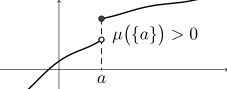
\includegraphics[height=2.3cm]{mira1}\hspace{10mm}
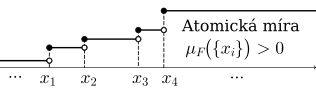
\includegraphics[height=2.3cm]{mira2}
\caption{Příklady různých $\mu$.}
\label{fig:mira1}
\end{figure}
\begin{dusl}
	Teorie míry: Pokud F splňuje D1 (monotonnost) a D2 (spojitost zprava), pak $\exists_1  \mu_F$ generovaná funkcí F tak, že $\mu((a,b])=F(b)-F(a)$, $\forall a<b$. Takto můžeme vytvořit Lebesgue-Stieltjesovu míru $\mu_F$. Pokud $\mu((a,b])=b-a$, $\forall a<b$, potom tuto míru nazveme Lebesgueovou mírou (lineární).
\end{dusl}
\begin{remark} Mějme $X\sim \PP^X$. Pak platí, že 
	\begin{enumerate}
		\item 	
		$ \PP(X=a)=\underbrace{\PP(x\leq a)}_{\FF_X(a)}-\underbrace{\PP(X<a)}_{*} = \FF_X(a)-\FF_X(a-) $ 
		$$ * = \PP\Bigl( \bigcup\limits_{n\geq 1}\underbrace{\{ X \leq a - \frac{1}{n} \}}_{A_n \nearrow A=\bigcup A_n} \Bigr)=\lim\limits_{n\to +\infty}\PP\Bigl( X \leq a - \frac{1}{n} \Bigr)=\lim\limits_{n\to +\infty}\FF_X\Bigl( a - \frac{1}{n} \Bigr) \equal{\text{ozn}}\FF_X(a-) $$ 
		Pokud je $\FF_X$ spojitá, pak $\PP(X=a)=\PP^X(\{a \})=0$.
		\item $ \PP(a\leq X \leq b)=\FF_X(b)-\underbrace{\PP(X<a)}_{\FF_X(a-)} $
		\item $ \PP(a\leq X < b)=\PP(X<b)-\PP(X<a)=\FF_X(b-)-\FF_X(a-) $
	\end{enumerate}
\end{remark}
\begin{theorem}
	Mějme $X\sim \PP^X~ (\FF_X)$. Pak $\FF_X$ má nejvýše spočetně mnoho skoků.
	\begin{proof}
		Definujeme $S_n:=\bigl\{ x:\FF_X $ má v $x$ skok větší, než $ \frac{1}{n} \bigr\}$. $S_n$ jsou konečné pro všechna $n\in\N$.
		$ S=\bigcup\limits_{n\geq 1}S_n $ má nejvýše spočetně prvků a obsahuje všechny skoky.
	\end{proof}
\end{theorem}
\begin{define} \label{diskretka}
	Nechť X je náhodná veličina s rozdělením $\PP^X$. X se nazývá \textbf{diskrétní náhodná veličina}, pokud je $\Ran(X) = \{ x_1,x_2,...,x_n,... \}$ nejvýše spočetná a předpokládáme, že $X^{-1}(\{ x_1,x_2,...,x_n,... \})=\Omega$. Značíme $(\forall k \in \hat{n},+\widehat{\infty})\bigl(p_k = \PP(X=x_k)\bigr)$. Definujeme
	\[
	f_X(x)=
	\begin{cases}
	p_k & x=x_k \\
	0 & x \neq x_k
	\end{cases} ~~~\forall k \in \hat{n},\widehat{+\infty}
	\]
	jako \textbf{diskrétní hustotu pravděpodobnosti} náhodné veličiny X (frekvenční funkci). \begin{remark}
	\begin{enumerate}
		\item 	Pro distribuční funkci diskrétní náhodné veličiny platí, že
	$$ \FF_X(x)=\PP(X\leq x)=\sum\limits_{k: x_k\leq x}\PP(X=x_k)= \sum\limits_{k=1}^{n,+\infty}\PP(X=x_k)\cdot \mathbb{I}_{[x_k,+\infty)}(x). $$
	\item $(\forall k\in\hat{n},+\widehat{\infty})\Bigl(f_X(x_k)=p_k\in [0,1]\Bigr)$
	\item $ \sum\limits_{k=1}^{n,+\infty}p_k=\PP(\Omega)=1$
	\item $\sum\limits_{k=1}^{n,+\infty}f_X(x_k)=1 $
	\end{enumerate}
	\end{remark}
\end{define}
\begin{example}
	\begin{enumerate}[a)]
		\item Rozdělení nazveme \textbf{Diracovo}, ozn. $X \sim \delta_c$, pokud $\PP(X=c)=1$.
		\item \textbf{Rovnoměrné rozdělení} náhodné veličiny X na $\{ x_1,...,x_m \}$ je rozdělení, pro které
		$$ \PP(X=x_k)=\frac{1}{m} ~~~\forall k \in \widehat{m} ~~\text{ a značíme ho }X \sim \bigcup\{ x_1,...,x_m \}.  $$
		\item Náhodná veličina $X$ má \textbf{Poissonovo rozdělení} s parametrem $\lambda>0$, značíme $X\sim \mathrm{Po}(\lambda) $, pokud 
		$$ \PP(X=k)=\frac{\lambda^k}{k!}\me^{-\lambda} ~~~\forall k\in\N $$
	\end{enumerate}
\end{example}
\begin{figure}[h]
	\centering
	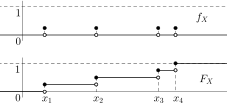
\includegraphics[width=0.55\linewidth]{rovnomdiskret}
	\caption{$f_X$ a $\FF_X$ pro rovnoměrné diskrétní rozdělení}
	\label{fig:rovnomdiskret}
\end{figure}
\begin{theorem}[Zákon řídkých jevů]
	Mějme sledovaný jev $A$ a čas $t\geq 0$ tak, že $t_0=0$. Označme $X_t$ jako počet událostí $($kdy nastal jev $A)$ do času $t\geq 0$. Nechť platí:\begin{enumerate}
		\item $X_{t+h} - X_t$ nezávisí na $X_t$
		\item $\PP(X_{t+h} - X_t=1)=\lambda h+o(h)$~~~při $h\to 0_+$ a $\lambda>0$, kde $\lim\limits_{ h\to 0+}\frac{o(h)}{h}=0$
		\item $\PP(X_{t+h}-X_t \geq 2)=o(h)$
		\item funkce $p_k(t)=\PP(X_t=k)$ je diferencovatelná vzhledem k $t$,~~~$\forall k \in \N$
	\end{enumerate}
Pak $(\forall t>0)(\forall k \in \N)\Bigl(\PP(X_t=k)=\frac{(\lambda t)^k}{k!}\me^{-\lambda t} \Bigr)$, což nazveme HPP (homogenní Poissonův proces) s intenzitou $\lambda>0$.
\begin{proof} Využijeme vztah $$\PP(X_{t+h}-X_t=0)=1-\PP(X_{t+h}-X_t=1)-\PP(X_{t+h}-X_t\geq 2)=1-\lambda h-o(h)+o(h).\text{ Pak}$$
	$$p_0 (t+h)=\PP(X_{t+h}=0)\equal{\text{nezáv}}\PP(X_t=0)\PP(X_{t+h}-X_t=0)=p_0(t)\br{1-\lambda h\underbrace{-o(h)+o(h)}_{o(h)}}~~~~/-p_0(t),~\cdot \frac{1}{h} $$
	$$ \frac{p_0(t+h)-p_0(t)}{h}=-\lambda p_0(t) + \frac{o(h)}{h} ~~~/ \lim\limits_{h\to 0+}$$
	$$ \dot{p}_0(t)=-\lambda p_0(t) $$
	$$
	p_k(t+h)=\sum\limits_{j=0}^k \underbrace{\PP(X_t=j)}_{p_j(t)}\PP(X_{t+h}-X_t=k-j)= \sum\limits_{j=0}^{k-2}p_j(t)o(h)~+p_{k-1}(t)\bigl(\lambda h +o(h)\bigr)~+p_k(t)\bigl(1-\lambda h+o(h)\bigr) 
	$$
	\begin{figure}[h]
		\centering
		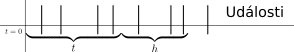
\includegraphics[width=0.6\linewidth]{udalosti}
		\label{fig:udalosti}
	\end{figure}
	$$ \frac{p_k(t+h)-p_k(t)}{h}=\sum\limits_{j=0}^{k-2}p_j(t)\frac{o(h)}{h}+\lambda p_{k-1}(t) + p_{k-1}(t)\frac{o(h)}{h}-\lambda p_k(t) + p_k(t)\frac{o(h)}{h}  ~~~/ \lim\limits_{h\to 0+}$$
	$$	\dot{p}_k(t) =\lambda p_{k-1}(t)-\lambda p_k(t),~~~k\geq 1$$
	Získali jsme tedy soustavu differenciálních rovnic
	\[ \begin{array}{ll}
	\dot{p}_0(t)=-\lambda p_0(t) & p_0(0)=1 \\
	\dot{p}_k(t) =\lambda p_{k-1}(t)-\lambda p_k(t)~~~~~ & p_k(0)=0
	\end{array} \]
	Čtenář může nyní ověřit, že tuto soustavu řeší rovnice $ p_k(t)=\PP(X_t=k)=\frac{(\lambda t)^k}{k!}\me^{-\lambda t} $.
\end{proof}
\end{theorem}
\begin{remark}
	Mějme náhodnou veličinu $ \X=(X_1,...,X_n)$. Řekneme, že $\X$ má \textbf{diskrétní rozdělení}, pokud $ \Ran(\X)=\{ \textbf{x}_1,...,\textbf{x}_k,... \}^{n,+\infty} $. Analogicky s definicí \ref{diskretka} pak
	$$ p_k=\PP(\X=\textbf{x}_k)=\PP(X_1=x_k^1,X_2=x_k^2,...,X_n=x_k^n),~~~k\geq 1 $$
	\[
	f(\textbf{x})=\begin{cases}
	p_k & \textbf{x}=\textbf{x}_k \\
	0 & \text{jinak}
	\end{cases}
	\]
\end{remark}
\begin{define}
	$ \X=(X,Y) $ náhodná veličina s DR. Pak definujeme \textbf{podmíněnou hustotu pravděpodobnosti} X za podmínky Y=y předpisem\[
	f_{X|Y}(x|y)=f_{X|Y=y}(x)=\frac{f_{(X,Y)}(x,y)}{f_Y(y)},
	\]
	pokud $ y \in \Ran(Y) $ a $ f_Y(y)> 0 $.
\end{define}
\begin{remark}
	$$ \frac{f_{(X,Y)}(x,y)}{f_Y(y)}= 	f_{X|Y}(x|y)=\frac{\PP(\overbrace{X=x}^{A},\overbrace{Y=y}^{B})}{\PP(Y=y)}=\frac{\PP(A\cap B)}{\PP(B)}=\PP(A|B)=\PP(X=x|Y=y) $$
\end{remark}







\chapter{Spojitá rozdělení}

\begin{define}
	Míra $\lambda$ je \textbf{$\sigma$-finitní} ($\sigma$-konečná), pokud $\exists(B_j)_{j=1}^{+\infty} \in \Bb_n$ tak, že $\Bigl(\bigcup\limits_{j=1}^{+\infty} B_j = \R^n \Bigr)$ a $(\forall j\in\N)\bigl(\lambda(B_j)<+\infty\bigr)$.
\end{define}
\begin{remark}
	 Lebesgueova míra $\lambda$ na ($\R,\Bb$) je $\sigma$-konečná, protože $\R=\bigcup\limits_{j=-\infty}^{+\infty}(j,j+1]$ a $\lambda\bigl((j,j+1]\bigr)=1$. Platí to i pro Lebesgueovu míru na ($\R^n,\Bb_n$).	
\end{remark}
\begin{define}\label{trhladefka}Pro míry $\nu,\lambda$ definujeme
	$$\nu\ll\lambda~\Leftrightarrow~(\forall \epsilon>0)(\exists \delta>0)(\forall B \in\Bb_n)\bigl(\lambda(B)<\delta~\Rightarrow~\nu(B)<\epsilon\bigr),$$ tedy pro $\nu$ konečnou je $\nu\ll \lambda$ ekvivalentní s $(\forall B \in\Bb)\bigl(\lambda(B)=0 ~\Rightarrow~ \nu(B)=0\bigr)$ a říkáme, že $\lambda$ \textbf{dominuje} $\nu$.
\end{define}
\begin{theorem}[o absolutně spojitém integrálu]
	Mějme borelovskou funkci $f\geq0$, $f\in\mathscr{L}^1(\R^n,\Bb_n,\lambda)$ a definujeme $$\nu(B):=\int_B f \dif\lambda,\text{ kde }\lambda\text{ je }\sigma\text{-konečná}. $$
	Pak $\nu\ll \lambda$, tedy platí, že $(\forall \epsilon>0)(\exists \delta>0)(\forall B\in\Bb_n)(\lambda(B)<\delta ~\Rightarrow~ \int_B f \dif\lambda < \epsilon)$.
\end{theorem}
\begin{dusl}[spojení]
	Nechť $\lambda$ je $\sigma$-finitní. Potom $\nu\ll \lambda~\Rightarrow~\exists_1  f\geq 0$ borelovská tak, že $$(\forall B\in\Bb_n)\bigl(\nu(B)=\int_B f \dif\lambda\bigr).$$
	\begin{proof}
			Mějme  $f,g:\R^n\to\R$ borelovské tak, že $f,g \geq 0$ a $\int_B g \dif\lambda = \nu(B)=\int_B f \dif\lambda$.\newline Volme pevné libovolné $\epsilon>0$ a sestrojme $B_\epsilon=\{ \textbf{x}:f(\textbf{x})+\epsilon\leq g(\textbf{x}) \}$, tedy platí, že
		$$ \int_{B_\epsilon} f\dif\lambda + \int_{B_\epsilon}  \epsilon \dif\lambda \leq \int_{B_\epsilon}  g \dif\lambda ~\Rightarrow~ \nu(B_\epsilon)+\epsilon\lambda(B_\epsilon)\leq \nu(B_\epsilon), ~~~\forall \epsilon>0.$$
		Z toho vyplývá, že $\epsilon\lambda(B_\epsilon)\leq 0$, tedy $\lambda(B_\epsilon)=0$. Potom sestrojme $\tilde{B}_\epsilon=\{ \textbf{x}:f(\textbf{x})-\epsilon\geq g(\textbf{x}) \}$:
		$$ \int_{\tilde{B}_\epsilon} f\dif\lambda - \int_{\tilde{B}_\epsilon}  \epsilon \dif\lambda \geq \int_{\tilde{B}_\epsilon}  g \dif\lambda ~\Rightarrow~ \nu(\tilde{B}_\epsilon)-\epsilon\lambda(\tilde{B}_\epsilon)\geq \nu(\tilde{B}_\epsilon), ~~~\forall \epsilon>0.$$
		Celkově tedy $\lambda(B_\epsilon)=0$ a $\lambda(\tilde{B_\epsilon})=0$. Protože toto platí pro všechna $\epsilon>0$, tak
		$$ \lambda(f<g)=0 ~\wedge ~\lambda(f>g)=0 ~~\Rightarrow~ ~\lambda(f=g)=0 $$
		Tímto jsme dokázali jednoznačnost. Důkaz existence je nad rámec předmětu 01MIP.
	\end{proof}
\end{dusl}
\begin{lemma}[Lebesgueova dekompozice konečné míry]\label{lebdekomp}
	Mějme konečné míry $\nu,\lambda$.\newline Potom $\exists f \geq 0$ borelovská a $\exists C \in\Bb_n$ tak, že $\lambda(C)=0$~~a~~$ \nu(B)=\int_B f \dif\lambda + \nu(B \cap C) $.
	\begin{proof}[Náznak důkazu]
		Ries-Fisherův reprezentační teorém (viz FA): $\mathcal{H}$ Hilbertův, na něm f lineární omezený funkcionál, pak $\exists_1  y \in\mathcal{H}$ tak, že $f(x)=\langle x|y\rangle$. Pro R-N.V. volíme $\mathcal{H}=L^2(\pi)$, kde $\pi=\nu+\lambda$.
	\end{proof}
\end{lemma}
\begin{theorem}[Radon-Nikodym]
	Nechť $ \nu $ a $ \lambda $ jsou dvě míry na $
	(\R^n,\Bb_n)$, $\lambda$ je $\sigma$-finitní a $\nu$ je absolutně spojitá vzhledem k míře $\lambda~(\nu\ll \lambda)$.\newline Potom $\exists f\geq 0,~f:\R^n\to\R$, borelovsky měřitelná funkce tak, že $(\forall B \in \Bb_n)\bigl(\nu(B)=\int_B f\dif\lambda\bigr)$.
	Navíc f je jednoznačná skoro všude v $\lambda$ a nazývá se Radon-Nikodymova derivace míry $\nu$ vzhledem k $\lambda$, ozn. $f=\frac{\dif\nu}{\dif\lambda}$.
	\begin{proof}
		 Mějme $\pi=\lambda+\nu$. Míra $\pi$ je $\sigma$-konečná, a proto $\exists(B_j)_{j=1}^{+\infty}$ tak, že $\bigcup\limits_{j=1}^{+\infty} B_j=\R^n$ a zároveň $\pi(B_j)<+\infty$. Pak ale $(\forall j\in\N)\bigl(\lambda(B_j)< +\infty~\wedge~\nu(B_j)<+\infty\bigr)$. Aplikujeme nyní lemma \ref{lebdekomp}: 
		 $$\exists f_j \geq 0\text{~~tak, že~~}\nu(B)=\int_{B} f_j \dif\lambda + \nu(B\cap C_j)\text{, ~~kde~~}\lambda(C_j)=0.$$ 
		 Dále zkonstruujeme $f=\sum\limits_{j=1}^{+\infty} \frac{1}{\lambda(B_j)}f_j \cdot \mathbb{I}_{B_j} $~a~$ C=\bigcup\limits_{j=1}^{+\infty} C_j$, pro kterou platí, že $ \lambda(C)=0 $.\newline Z předpokladu víme, že $\nu\ll \lambda$ a $\nu$ je konečná. Z definice \ref{trhladefka} potom vyplývá, že \newline$(\forall B \in\Bb_n)\bigl(\lambda(B)=0 ~\Rightarrow~ \nu(B)=0\bigr)$, takže
		 $$\lambda(C)=0~~\Rightarrow~~0\leq \nu(B\cap C) \leq \nu(C)=0 ~~\Rightarrow~ ~\nu(B\cap C)=0.$$	\end{proof}
\end{theorem}
\begin{remark}
	Mějme $\nu=\PP^\X$ jako rozdělení náhodné veličiny $\X=(X_1,...,X_n),$\newline$\X:\Omega\to\R^n$, a nechť $\lambda$ je $\sigma$-konečná. Pak $$\PP^\X\ll \lambda~~\Leftrightarrow ~~\exists_1  \fex\geq 0\text{ borelovská} ~\wedge ~(\forall B \in\Bb_n)\bigl(\PP^\X(B)=\int\limits_{B}\fex \dif\lambda\bigr).$$
\end{remark}
\begin{remark}
	Libovolná funkce $f\geq 0,~ \int\limits_{\R^n} f \dif\lambda=1$ definuje pravděpodobnostní míru $ \PP_f(B)=\int\limits_Bf\dif\lambda.$ Splňuje přitom $\sigma$-aditivitu.
\end{remark}
%\begin{remark} $$ \nu((-\infty,\textbf{x}])=\int\limits_{-\infty}^\textbf{x}f \dif\lambda + \nu_\perp^\text{diskr}((-\infty,\textbf{x}])+ \nu_\perp^\text{spoj.}((-\infty,\textbf{x}]) $$ $$ \FF_X(\textbf{x})=\FF_{AS}(\textbf{x})+\FF_Y(\textbf{x})+\FF_{SS}(\textbf{x}) $$ $\FF_Y(\textbf{x})$ je skoková s nejvýše spočetně skoky\end{remark}
\begin{define}
Řekneme, že náhodná veličina $\X\sim \PP^\X$ má $ASR_\lambda$ (\textbf{absolutně spojité rozdělení} vzhledem k $\lambda$), pokud $\PP^\X\ll \lambda$, kde $\lambda$ je $\sigma$-konečná, a pokud existuje právě jedna $\fex:\R^n\to\Rop$ taková, že $\PP(\X\in B) = \PP^\X(B)=\int\limits_{B} \fex \dif\lambda~~\forall B\in\Bb_n$. Funkci $\fex$ nazýváme \textbf{hustotou pravděpodobnosti} (pdf/PDF) náhodné veličiny $\X$.
\end{define}
\begin{remark}
	$$ \PP(\X\leq \textbf{b})= \PEX\Bigl(\bigtimes\limits_{i=1}^n(-\infty,b_i]\Bigr)=\int\limits_{\bigtimes\limits_{i=1}^n(-\infty,b_i]} \fex(\textbf{x})\dif\lambda=\int\limits_{-\infty}^{b_1}...\int\limits_{-\infty}^{b_n}\fex(\textbf{x})\underbrace{\dif\textbf{x}}_{\dif\lambda = \dif x_1\dif x_2...\dif x_n} $$
	$$ \PP(a<\X\leq \textbf{b})=\int\limits_{a_1}^{b_1}...\int\limits_{a_n}^{b_n}\fex(\textbf{x})\dif\textbf{x} $$
\end{remark}

\begin{remark}
Vlastnosti $\fex$: \begin{enumerate}
	\item $\fex \geq 0$
	\item $\int\limits_{\R^n} \fex \dif\lambda = \PP^\X(\R^n)=1$
	\item $\PP^\X(B) = \int\limits_B \fex \dif\lambda$
\end{enumerate}
\end{remark}

\begin{theorem}
	Nechť $\X\sim\PEX$ a $\lambda$ je $\sigma$-konečná. Pak 
	$$\PEX \ll  \lambda ~(\X\text{ má ASR}_\lambda) ~\Leftrightarrow ~(\exists_1 \fex\geq 0\text{ borelovská})(\forall \textbf{x}\in\R^n)\Bigl(\FEX(\textbf{x})=\int\limits_{-\infty}^{x_1}...\int\limits_{-\infty}^{x_n}\fex(\textbf{t})\dif\textbf{t}\Bigr).$$
	\begin{proof}
		\begin{enumerate}[$\Rightarrow$:]
			\item R-N. V. + zúžení na $\tau_{1,n}$
		\end{enumerate}
	\begin{enumerate}[$\Leftarrow$:]
	\item Máme tedy $\fex$. Definujeme dále $\PP'(B):=\int\limits_{B}\fex \dif\textbf{x}$. Pro ni ukážeme, že se jedná o pravděpodobnost: \begin{enumerate}[1)]
		\item $\PP'(B)\geq0$
		\item $\PP'(\R^n)=\int\limits_{\R^n}\fex \dif\textbf{x}=\lim\limits_{\substack{x_i \to +\infty \\ \forall i\in\hat{n}}}\int\limits_{-\infty}^{x_1}...\int\limits_{-\infty}^{x_n}\fex(\textbf{x})\dif\textbf{x}=\lim\limits_{\substack{x_i \to +\infty \\ \forall i\in\hat{n}}}\FEX(\textbf{x})=1$
		\item $\PP'\Bigl(\sum\limits_{j=1}^{+\infty} B_j\Bigr)=\int\limits_{\sum\limits_{j=1}^{+\infty} B_j}\fex \dif\textbf{x}\equal{\text{Leb.~int.}}\sum\limits_{j=1}^{+\infty} \int\limits_{B_j}\fex \dif\textbf{x}=\sum\limits_{j=1}^{+\infty} \PP'(B_j)$
	\end{enumerate}
\[\left.
\begin{array}{l}
P'\text{ je pravděpodobnost na }(\R^n,\Bb_n)
\\ 
\PEX\text{ je pravděpodobnost na }(\R^n,\Bb_n)
\end{array}\right\} ~\Rightarrow~\text{ na }\tau_{1,n}\text{ splývají }\PP'=\PEX
\]
$\tau_{1,n}=\{ \bigtimes\limits_{j=1}^n (-\infty,x_j]:x_j\in\R \}$ je uzavřený na konečné průniky a $\sigma(\tau_{1,n})=\Bb~\stackrel{\ref{Veta226}}{\Longrightarrow}~ \PEX = \PP'$ na celém ($\R^n,\Bb_n$).
\end{enumerate}
	\end{proof}
\end{theorem}
\begin{remark}
Platí, že
$$ \fex(\textbf{x}_0)=\frac{\partial \FEX}{\partial x_1...\partial x_n}(\textbf{x}_0) \text{, ~kde }\textbf{x}_0\text{ je bod spojitosti }\fex. $$
\end{remark}
\begin{theorem}
	Mějme $\X\sim\PEX$ s ASR$_\lambda$ $(\lambda$ - Lebesgue$)$ $($zapisujeme $\X\sim\fex)$, ozn.\newline $\X'=(X_1,...,X_{j-1},X_{j+1},...,X_n)$. Pak $\X'$ má ASR a platí, že $$f_{\X'}(\textbf{x}')=\int\limits_{-\infty}^{+\infty}\fex(\textbf{x}) \dif x_j~~~\forall \textbf{x}'\in\R^{n-1}$$
	\begin{proof}
		\[
		\begin{split}
		\FF_{\X'}(\textbf{x}')&=\lim\limits_{x_j\to+\infty}\FEX(\textbf{x})=\lim\limits_{x_j\to+\infty}\int\limits_{-\infty}^{x_1}...\int\limits_{-\infty}^{x_j}...\int\limits_{-\infty}^{x_n}\fex(\textbf{t})\dif\textbf{t}\equal{\text{F.V.}}\lim\limits_{x_j\to+\infty}\int\limits_{-\infty}^{x_j}\int\limits_{-\infty}^{x_1}...\int\limits_{-\infty}^{x_{j-1}}\int\limits_{-\infty}^{x_{j+1}}...\int\limits_{-\infty}^{x_n}\fex \dif\textbf{t}= \\ &=\int\limits_{-\infty}^{+\infty}\int\limits_{-\infty}^{x_1}...\int\limits_{-\infty}^{x_{j-1}}\int\limits_{-\infty}^{x_{j+1}}...\int\limits_{-\infty}^{x_n}\fex \dif\textbf{t}\equal{\text{F.V.}}\int\limits_{-\infty}^{x_1}...\int\limits_{-\infty}^{x_{j-1}}\int\limits_{-\infty}^{x_{j+1}}...\int\limits_{-\infty}^{x_n}\underbrace{\int\limits_{-\infty}^{+\infty} \fex(\textbf{t})\dif t_j}_{f_{\X'\text{ je pdf k }\X'}} \dif t_1...\dif t_n
		\end{split}
		\]
	\end{proof}
\end{theorem}
\begin{remark}
Speciálně pro n=2:
	\[
	\begin{split}
	(X,Y)\sim f_{X,Y} &~\Rightarrow~ f_Y(y)=\int\limits_{-\infty}^{+\infty}f_{X,Y}(x,y)\dif x ~~~(\text{marginální hustota pravděpodobnosti Y}) \\
	&~\Rightarrow~ f_X(x)=\int\limits_{-\infty}^{+\infty}f_{X,Y}(x,y)\dif y 
	\end{split}
	\] 
	Zobecněně:
	Mějme $\{ i_1,...,i_k \} \subset \hat{n},~k<n$~~a~~$\{ i_{k+1},...,i_n \}$ doplněk do $\hat{n}$, $\X\sim\fex$ (ASR). Pak $$f_{(X_{i_1},...,X_{i_k})}(x_{i_1},...,x_{i_k})=\int\limits_{-\infty}^{x_{i_{k+1}}}...\int\limits_{-\infty}^{x_{i_{n}}}\fex(\textbf{t})\dif t_{i_{k+1}}...\dif t_{i_{n}}$$
\end{remark}
\begin{theorem}
	Mějme $\X\sim\PEX$ s ASR $(\fex)$. Pak
	$$X_1,... ,X_n\text{ jsou stochasticky nezávislé}~\Leftrightarrow ~\fex(\textbf{x})=\prod\limits_{j=1}^n f_{X_j}(x_j)~~\forall \textbf{x}\in\R^n.$$
	\begin{proof}
		\begin{enumerate}[$\Rightarrow$:]
			\item $$X_1,... ,X_n\text{ nezávislé}~\Leftrightarrow ~\FEX(\textbf{x})\stackrel{\forall \textbf{x}}{=}\prod\limits_{j=1}^n \FF_{X_j}(x_j)\equal{\text{ASR}}\prod\limits_{j=1}^n \int\limits_{-\infty}^{x_j} f_{X_j}(t_j)\dif t_j\equal{\text{F.V.}}\int\limits_{-\infty}^{x_1}... \int\limits_{-\infty}^{x_n}\prod\limits_{j=1}^n f_{X_j}(t_j)\dif\textbf{t}$$
		\end{enumerate}
	\begin{enumerate}[$\Leftarrow$:]
	\item $$\PP(X_j\in \underbrace{B_j}_{\in\Bb_1},~ \forall j \in \hat{n})\equal{\text{R-N.V.}}\int\limits_{\bigtimes\limits_{j=1}^n B_j} \fex(\textbf{x})\dif\textbf{x}=\int\limits_{\bigtimes\limits_{j=1}^n B_j} \prod\limits_{j=1}^n f_{X_j}(x_j)\dif\textbf{x}\equal{\text{F.V.}}\prod\limits_{j=1}^n \underbrace{\int\limits_{B_j}f_{X_j}(x_j)\dif x_j}_{\PP(X_j\in B_j)} $$
\end{enumerate}
	\end{proof} 
\end{theorem}
\begin{define}
	Nechť $(X,Y)$ je náhodná veličina s ASR $(f_{(X,Y)})$. Definujeme podmíněnou hustotu náhodné veličiny $X$ za předpokladu $Y=y$ pro pevné $y\in\Ran(Y)$ tak, že $f_Y(y)\neq 0$, vztahem
	$$f_{X|Y}(x|y):=\frac{f_{X,Y}(x,y)}{f_Y(y)} ~~~\forall x\in\R.$$
\end{define}
\begin{remark}
	Korektnost definice:
	\begin{enumerate}
		\item $f_{X|Y}\geq 0$
		\item $\int\limits_{-\infty}^{+\infty}f_{X|Y}(x|y)\dif x=\frac{1}{f_Y(y)}\int\limits_{-\infty}^{+\infty}f_{X,Y}(x,y)\dif x=\frac{f_Y(y)}{f_Y(y)}=1$
	\end{enumerate}
Díky tomu můžeme pro $B\in\Bb_1$ definovat $\PP^{X|Y}(B)=\int\limits_{B} f_{X|Y}(x|y)\dif x$ jako pravděpodobnostní míru a označíme $X|Y(=y)\sim \PP^{X|Y(=y)}$.
\end{remark}
\begin{theorem}
	Mějme náhodnou veličinu $\X=(X_1,... ,X_n)$ $\sim\fex$ (ASR) a nechť $g:\R^n\to\R^m$ je borelovsky měřitelná funkce. Definujeme dále $\mathbb{Y}=g(\X)$. Pak 
	$$f_\mathbb{Y}(\textbf{y})=\frac{\partial^m}{\partial y_1... \partial y_m}\int\limits_{B_\textbf{y}}\fex(\textbf{x})\dif\textbf{x},~~~B_\textbf{y}:=\{ \textbf{x}:g(\textbf{x})\leq \textbf{y} \} \in\Bb.$$
	\begin{proof}Definujme $B_\textbf{y}:=\{ \textbf{x}:g(\textbf{x})\leq \textbf{y} \} \in\Bb$. Pak
	\[
	\begin{split}
	\FF_\mathbb{Y}(\textbf{y})&=\PP(\mathbb{Y}\leq \textbf{y})=\PP(g\circ \X\leq \textbf{y})=\PP\Bigl(\underbrace{(g \circ \X)^{-1}}_{\X^{-1}\circ g^{-1}}\bigl((-\infty,\textbf{y}] \bigr)\Bigr)=\PEX \Bigl(g^{-1}\bigl((-\infty,\textbf{y}]\bigr)\Bigr) \equal{\text{ASR}}\int\limits_{B_\textbf{y}}\fex \dif\textbf{x} \\ f_\mathbb{Y}(\textbf{y})&=\frac{\partial^m}{\partial y_1... \partial y_m}\FF_\mathbb{Y}(\textbf{y})~s.v.~~~~~(pozn.~~\FF_\mathbb{Y}(\textbf{y})=\int\limits_{-\infty}^{y_1}... \int\limits_{-\infty}^{y_m}f_\mathbb{Y} \dif\textbf{y}) 
	\end{split}
	\]
	\end{proof}
\end{theorem}
\begin{theorem}
	Mějme $\X\sim \fex$ (ASR) a $g:\R^n\to\R^n$ borelovskou tak, že $g$ je na (částech) $B_i$ regulární a prostá $\forall i \in \hat{k}$. Nechť $B_i\subset \R^n$ jsou otevřené a disjunktní a $G:=\sum\limits_{i=1}^k B_i$ je takové, že $\int\limits_{G}\fex \dif\textbf{x}=1$, tedy $\PEX(G)=1$. Pak $\Y =g(\X)$ má ASR a platí pro něj, že
	$$\fey(\textbf{y})=\begin{cases}
	\sum\limits_{i=1}^k \fex\bigl(g_i^{-1}(\textbf{y})\bigr)\left| \mathbb{J}_{g_i^{-1}}(\textbf{y}) \right| &\textbf{y}\in g(G), \\ 0 & \text{jinde,}
	\end{cases}$$
	  kde $g_i^{-1}$ jsou funkce inverzní k $g$ na $B_i$ pro $\forall i\in\hat{k}$.
	\begin{center}
		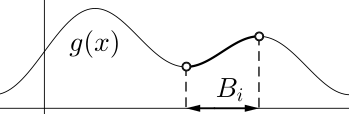
\includegraphics[width=0.24\linewidth]{opendiscret}
	\end{center}
	\begin{proof}Označme opět $B_\textbf{y}:=\{ \textbf{x}:g(\textbf{x})\leq \textbf{y} \}$. Pak
		\[
		\begin{split}
		&\FEY(\textbf{y})=... =\int\limits_{B_\textbf{y}}\fex(\textbf{x})\dif\textbf{x} =\int\limits_{B_\textbf{y}\cap \sum\limits_{i=1}^k B_i}\fex(\textbf{x})\dif\textbf{x}=\sum\limits_{i=1}^k \int\limits_{B_\textbf{y}\cap B_i} \fex(\textbf{x}) \dif\textbf{x}= \begin{array}{|c|}
		 g(\textbf{x})=\textbf{t}\\ 
		\textbf{x}=g_i^{-1}(\textbf{t})\text{ na }B_i\\ 
		\mathbb{J}_{g_i^{-1}}(\textbf{t})\neq 0
		\end{array} = \\
		&= \sum\limits_{i=1}^k \int\limits_{\{ \textbf{t}:\textbf{t}\leq \textbf{y} \}\cap g(B_i)}\fex\bigl(g_i^{-1}(\textbf{t})\bigr)\left| \mathbb{J}_{g_i^{-1}}(\textbf{t}) \right|\dif\textbf{t}=\int\limits_{-\infty}^{y_1}... \int\limits_{-\infty}^{y_n}\sum\limits_{i=1}^k \fex(g_i^{-1}(\textbf{t}))\left| \mathbb{J}_{g_i^{-1}}(\textbf{t}) \right|\dif\textbf{t}=\int\limits_{-\infty}^{y_1}... \int\limits_{-\infty}^{y_n}\fey(\textbf{t})\dif\textbf{t} ,
		\end{split}
		\]
		tedy $\fey$ je hustota pravděpodobnosti $\Y$.
	\end{proof}
\end{theorem}
\begin{dusl}~
	\begin{enumerate}[a)]
		\item Mějme speciální případ $n=1$, $X\sim \fex $ (ASR), $g$ ryze monotonní, $\exists g'\in\mathcal{C}^1$, $g'\neq 0$ na $B_i$ $\forall i\in\hat{k}$ (disjunktní intervaly). Pak $$Y=g(X)\text{ má ASR ~~a~~ }f_Y(y)=\sum\limits_{i=1}^k f_x (g_i^{-1}(y))\frac{1}{\left| g_i'(g_i^{-1}(y)) \right|}~~~(\text{derivace inverzní funkce})$$
		\item $k=1$:~~ $\fey(\textbf{y})=\fex(g^{-1}(\textbf{y}))\left| \mathbb{J}_{g^{-1}}(\textbf{y}) \right|$ ~~~$\forall \textbf{y}\in g(G)$
		\item Mějme $g:\R^n\to\R^1$, $y_1=g(x_1,... ,x_n)$ tak, že lze jednoznačně vyjádřit $x_1$ pomocí $y_1$ a $(x_2,... ,x_n)$. Označme $x_1=h(y_1,\underbrace{\textbf{x}'}_{=(x_2,... ,x_n)})=h(\textbf{y})$, $y_2=x_2$, $y_3=x_3$, ...,  $y_n=x_n$ 
		a předpokládejme, že $\exists \frac{\partial h}{\partial y_1}(\textbf{y})$ spojitá a nenulová. Tím jsme definovali $\tilde{g}:\R^n\to\R^n$ (prostou): $$\mathbb{J}_{\tilde{g}^{-1}}=\left| \begin{array}{cccc}
		\frac{\partial h}{\partial y_1} & \mathbb{O} \\ 
		\mathbb{O}&  \mathbb{I}_{n-1}
		\end{array}\right|= \frac{\partial h}{\partial y_1}\neq 0.$$
		\[
		\begin{split}
		\fey(\textbf{y})&=\fex\bigl(\tilde{g}^{-1}(\textbf{y})\bigr) \left| \mathbb{J}_{\tilde{g}^{-1}}(\textbf{y}) \right|=\fex\bigl(h(y_1,\underbrace{\textbf{x}'}_{=y_2,... ,y_n}),y_2,... ,y_n\bigr)\left| \frac{\partial h}{\partial y_1}(y_1,y_2,... ,y_n) \right|= \\ &= \fex\bigl(h(\textbf{y}),y_2,... ,y_n\bigr) \left| \frac{\partial h}{\partial y_1}(\textbf{y}) \right|~~~\Rightarrow~ ~~f_{Y_1}(y_1)=\int \fey (\textbf{y})\dif y_2... \dif y_n 
		\end{split}
		\] 
	\end{enumerate}
\begin{enumerate}[c2)]
	\item Označme $X_1=X$, $X_2=Y$, $(X,Y)\stackrel{ASR}{\sim}f_{(X,Y)}$. Trasformace $\begin{array}{|c|}
	U=X+Y	\\ V=Y
	\end{array}: ~ \R^2\to\R^2$ \newline 
	$	u=x+y,~u:\R^2\to\R^1~~\Rightarrow~~ x=u-y=:h(u,y)~\Rightarrow~~ \frac{\partial h}{\partial u}=1  $
	$$ f_{u,v}(u,v)=f_{X,Y}(u-v,v)\cdot 1 $$
	$$ f_{X+Y}(u)=f_U(u)=\int\limits_{-\infty}^{+\infty} f_{X,Y}(u-v,v)\dif v\equal{\text{id}}\int\limits_{-\infty}^{+\infty} f_X(u-v)f_Y(v)\dif v=f_X \ast f_Y $$
\end{enumerate}
\begin{enumerate}[c3)]
	\item Mějme $(X,Y)\sim f_{X,Y} $ a označme  $ U=X\cdot Y$ $$ x=\frac{u}{y}=\frac{u}{v}=:h(u,v)~\Rightarrow~ \frac{\partial h}{\partial u}=\frac{1}{v},~v\neq 0 $$
	$$f_{X\cdot Y}(u)= f_U(u)=\int\limits_{-\infty}^{+\infty} \frac{1}{|v|}f_{X,Y}\left(\frac{u}{v},v\right)\dif v\equal{\text{id}}\int\limits_{-\infty}^{+\infty} \frac{1}{|v|}f_X\left( \frac{u}{v} \right)f_Y(v)\dif v $$
\end{enumerate}
\end{dusl}
\begin{define}
	Řekneme, že $X\sim U(a,b)$, $a<b$, má\textbf{ uniformní rozdělení} na intervalu $(a,b)$, pokud $f_X(x)=\frac{1}{b-a}$, $x\in/a,b/$. (je jedno o které závorky se jedná)
\end{define}	
\begin{define}
	Mějme $X\sim U(G)$ (uniformní rozdělení), kde $G\subset \R^n$ a $\lambda(G)<+\infty$. Pak definujeme $\fex(\textbf{x}):=\frac{1}{\lambda(G)}$ na $G$. ($\int\limits_{-\infty}^{+\infty}\fex \dif\lambda=\int\limits_{G}\frac{1}{\lambda(G)}\dif\lambda=1$)
\end{define}
\begin{define}[Gaussovo rozdělení]
	Definujeme Gaussovo rozdělení, ozn. $X\sim \mathrm{N}(\mu,\sigma^2)$, $(\mu\in\R,\sigma>0)$, pomocí vztahů  \[
	\begin{split}
	f_X(x)&=\frac{1}{\sqrt{2 \pi\sigma^2}}\me^{-\frac{1}{2 \sigma^2}(x-\mu)^2},~~~ x\in\R,~\mu\in\R,~\omega^2>2 \\  \FF_X(x)&=\frac{1}{\sqrt{2 \pi\sigma^2}}\int\limits_{-\infty}^x \me^{-\frac{1}{2 \sigma^2}(t-\mu)^2} \dif t,~~~ \FF_X(+\infty)=1
	\end{split}
	\]
\end{define}
\begin{define}
	Gaussovo rozdělení pro $\sigma=1$ a $\mu=0$ $\br{X\sim \mathrm{N}(0,1)}$ označujeme
	\[
	\begin{split}
	\phi(x)&:=\frac{1}{\sqrt{2 \pi}}\me^{-\frac{x^2}{2 }}, \\
	\Phi(x)&:=\frac{1}{\sqrt{2\pi}}\int\limits_{-\infty}^x \me^{-\frac{t^2}{2}}\dif t.
	\end{split}
	\]
\end{define}
\begin{theorem}\label{N}
	\begin{enumerate}
		\item $\mathrm{N}(\mu,\sigma^2)$ je symetrické rozdělení okolo $\mu$, $\mathrm{N}(0,1)$ je symetrické okolo 0
		\item $\Phi(x)=1-\Phi(-x)$,~~~$\forall x \in\R$
		\item $f_{\mathrm{N}(\mu,\sigma^2)}(x)=\frac{1}{\sigma}\varphi\left(\frac{x-\mu}{\sigma}\right) $ $$\FF_{\mathrm{N}(\mu,\sigma^2)}(x)=\frac{1}{\sqrt{2\pi\sigma^2}}\int\limits_{-\infty}^x \me^{-\frac{1}{2 \sigma^2}(t-\mu)^2}\dif t=\left| \frac{t-\mu}{\sigma}=u \right|=\frac{1}{\sqrt{2\pi}}\int\limits_{-\infty}^{\frac{x-\mu}{\sigma}}\me^{-\frac{\mu^2}{2}}du=\Phi\left(\frac{x-\mu}{\sigma}\right)$$ 
		\item $\PP(a<X\leq b)=\FF_X(b)-\FF_X(a)=\Phi\Bigl(\underbrace{\frac{b-\mu}{\sigma}}_{d}\Bigr)-\Phi\Bigl(\underbrace{\frac{a-\mu}{\sigma}}_{c}\Bigr)=\frac{1}{\sqrt{2\pi}}\int\limits_{c}^d \me^{-\frac{x^2}{2}}\dif x$
		\item $X\sim \mathrm{N}(\mu,\sigma^2)~\Rightarrow~ \underbrace{aX+b}_{Y} \sim \mathrm{N}(a\mu+b,a^2\sigma^2)$, $a\neq 0$
		\[
		\begin{split}
		f_Y(y)&=f_X\bigl(g^{-1}(y)\bigr)\bigl|\mathbb{J}_{g^{-1}}(y)\bigr|=\left| \begin{array}{c}
		g: y=ax+b	\\ 
		g^{-1}:x=\frac{y-b}{a}	\\ 
		\mathbb{J}_{g^{-1}}(y)=\frac{1}{a}
		\end{array}  \right|=\frac{1}{|a|}\frac{1}{\sqrt{2\pi}~\sigma}\me^{-\frac{1}{2\sigma^2}(\frac{y-b}{a}-\mu)^2}=\\
		&=\frac{1}{\sqrt{2\pi}\underbrace{|a|\sigma}_{\sigma'}}\me^{-\frac{1}{2a^2\sigma^2}(y-\overbrace{(a\mu+b)}^{\mu'})^2}\sim \mathrm{N}(\mu',\sigma'^2) 
		\end{split}
		\] 
		\item $X\sim \mathrm{N}(\mu,\sigma^2)~\Rightarrow~ \frac{X-\mu}{\sigma}\sim \mathrm{N}(0,1)$ \newline
		$X\sim \mathrm{N}(0,1)~\Rightarrow~ \sigma X+\mu \sim \mathrm{N}(\mu,\sigma^2)$
		\item $$ \PP(\mu-k \sigma\leq X \leq \mu+k \sigma)\equal{k\in\N}\PP\Bigl(-k\leq \underbrace{\frac{X-\mu}{\sigma}}_{\mathrm{N}(0,1)}\leq k\Bigr)=\Phi(k)-\underbrace{\Phi(-k)}_{1-\Phi(k)}=-1+2\Phi(k)=\begin{cases}
		0.6827 & k=1 \\ 0.9545 & k=2 \\ 0.9973 & k=3 \\ ... 
		\end{cases} $$
	\end{enumerate}
\end{theorem}
\begin{remark}
	Degenerovanou $\mathrm{N}(\mu,0)\:=\delta_\mu$ - Dirac v bodě $\mu$ (diskrétní)
\end{remark}
\begin{theorem}[Reprodukce]
	Mějme $(X_j)_1^n\sim \mathrm{N}(\mu_j,\sigma_j^2)$ nezávislé $(\text{id})$, $\textbf{a}=(a_j)_{j=1}^n\neq \textbf{0}$. Pak $$\sum\limits_{j=1}^n a_jX_j\sim N\left( \sum\limits_{j=1}^n a_j\mu_j,\sum\limits_{j=1}^na_j^2\sigma_j^2 \right)$$
	\begin{proof}
		Z věty \ref{N} víme, že $(\forall j\in\N)\Bigl(a_jX_j\sim \mathrm{N}(a_j\mu_j,a_j^2\sigma_j^2)\Bigr)$. Následně postupujeme indukcí:\newline 
		n=2: \[
		\begin{split}
		X_1+X_2\sim f_{X_1+X_2}(u)&\equal{\text{id}}(f_{X_1}\ast f_{X_2})(u)=\int\limits_{-\infty}^{+\infty} f_{X_1}(u-v)f_{X_2}(v)\dif v=\\ &=\frac{1}{2\pi\sigma_1\sigma_2}\int\limits_{-\infty}^{+\infty} \me^{-\frac{1}{2\sigma_1^2}(u-v-\mu_1)^2-\frac{1}{2\sigma_2^2}(v-\mu_2)^2}\dif v=...  \sim \mathrm{N}(\mu_1+\mu_2,\sigma_1^2+\sigma_2^2)
		\end{split} \]
		$n\to n+1$: $$ \sum\limits_{j=1}^{n+1}X_j=\sum\limits_{j=1}^n X_j + X_{n+1} \sim N\Bigl(\sum\limits_{j=1}^n \mu_j + \mu_{n+1},\sum\limits_{j=1}^n \sigma_j^2+\sigma_{n+1}^2\Bigr) $$
	\end{proof}
\end{theorem}
\begin{remark}
	\begin{enumerate}
		\item 	$$a=\left( \frac{1}{n},... ,\frac{1}{n} \right)~\Rightarrow~ \frac{1}{n}\sum\limits_{j=1}^n X_j = \overline{X}_n \sim N\Bigl( \underbrace{\bar{\mu}_n}_{\frac{1}{n}\sum\limits_{j=1}^n \mu_j},\frac{1}{n}\underbrace{\bar{\sigma}_n^2}_{\frac{1}{n}\sum\limits_{j=1}^n \sigma_j^2 (i.i.d.)} \Bigr)\equal{
			\mu_j=\mu,~\sigma_j=\sigma }N\left( \mu,\frac{1}{n}\sigma^2 \right)$$
	
\item $X\sim \mathrm{N}(0,1)~\Rightarrow~ X^2\sim \chi^2(1)$ - Rozdělení chí kvadrát
\item $X\sim \mathrm{N}(\mu,\sigma^2)~\Rightarrow~ \me^X \sim \mathrm{LN}(\mu,\sigma^2)$ - log-normální rozdělení
\item $X,Y ~i.d.~\mathrm{N}(0,1)~\Rightarrow~ \frac{X}{Y}\sim C(0,1) $ - Cauchyho rozdělení
\item $ X_j ~i.i.d.~\mathrm{N}(0,1)~\Rightarrow~ Y=\sum\limits_{j=1}^n X_j^2 \sim \chi^2(n),~(g(\textbf{x})=\textbf{y}:\R^n\to\R^1)$
\item $X\sim \mathrm{N}(0,1)\wedge Y\sim \chi^2(n)$ nezávislý $~\Rightarrow~\frac{X}{\sqrt{\frac{Y}{n}}}\sim \frac{\mathrm{N}(0,1)}{\sqrt{\frac{\chi^2(n)}{n}}}\equal{\text{id}}t(n)$ - Studentovo rozdělení
\item $X\sim \chi^2(n) \wedge~Y\sim \chi^2(m)$ nezávislý $~\Rightarrow~ \frac{\frac{X}{n}}{\frac{Y}{m}}\sim F(n,m)$ - Fisherovo-Snedecorovo rozdělení
\end{enumerate}
\end{remark}
\begin{define}
	Říkáme, že $\X$ má \textbf{rozdělení z exponenciální třídy}, pokud \newline $\X\sim f(\textbf{x})=h(\textbf{x})c(\Theta)\me^{Q(\Theta)\cdot T(\textbf{x})}$,~~~$\forall \textbf{x}\in\R^n,~ \Theta\in\R^k$, kde \begin{enumerate}
		\item $h:\R^n\to\R_0^+,$
		\item $c(\Theta)\in\R^+$ je normovací konstanta, $c(\Theta)=\int\limits_{\R^n}h\me^{Q\cdot T}\dif\textbf{x}<+\infty$
		\item $Q:\R^k\to\R^k,~T:\R^n\to\R^k,~k<n$
	\end{enumerate}
\end{define}
